%
% teil3.tex -- Beispiel-File für Teil 3
%
% (c) 2020 Prof Dr Andreas Müller, Hochschule Rapperswil
%
% !TEX root = ../../buch.tex
% !TEX encoding = UTF-8
%


\section{Harmonische Systeme und Rauschen\label{brown:Rauschen}}
\rhead{Implikationen}

Um dem Thema des Buches gerecht zu werden und dieses Kapitel einzugliedern, kann die harmonische Analysis als essenzielles Werkzeug betrachtet werden, um mit Rauschen umzugehen und dieses zu charakterisieren. 

So ist die "Fast Fourrier Transform" eine wichtige Methode, um periodische Signale von Rauschen unterscheiden zu können.
Weiter können mittels harmonischer Analysis auch Filter entwickelt werden, welche ein Signal von Rauschen befreien. Ein gutes Beispiel dafür sind Bandpassfilter, welche nur ein bestimmtes Band an Frequenzen durchlassen.

Für viele Anwendungen ist es auch möglich mittels hochfrequenter überlagerten Schwingungen Rauschen zu modellieren. Dies ist natürlich nur eine Annäherung, da "echtes" Rauschen - je nach Fachbereich und Definition - weder vorhersagbar sein sollte, noch Information beinhaltet. 

Durch die Analyse von Systemantworten auf verschiedene harmonische Anregungen kann eine Aussage getroffen werden, wie das System auf Rauschen - also eine zufällige Störung - reagieren könnte.

All diese Beispiele basieren auf Methoden der Harmonischen Analysis. Um den Bogen zur Anfangsbemerkung dieses Kapitels zu schliessen: Durch Zufälle kann Rauschen entstehen, was meist ungewollt ist. Rauschen kann als "Gegenteil" der harmonischen Analysis erachtet werden, obwohl dafür keine klare mathematische Definition besteht. Dank Methoden der hamronsichen Analysis ist es möglich diese gegenteiligen Eigenschaften zu untersuchen und zu bewerten.

- Differenzierbarkeit



\subsection{Was ist Rauschen?\label{brown:Rauschen:Arten}}
Rauschen ist in vielen technischen und wissenschaftlichen Disziplinen ein wichtiger Faktor. So kann es auch in verschiedenen Kontexten unterschiedlich definiert werden. 
Zum Beispiel in der Signal- und Kommunikationstechnik kann Rauschen als zufällige, unvorhersehbare und auch ungewollte Fluktuation beschrieben werden. 

Mathematisch können unterschiedliche Arten von Rauschen beschrieben werden, einige der wichtigsten sind folgende: 


\textbf{Weisses Rauschen:}
	\begin{itemize}
	\item Alle Frequenzkomponenten haben die gleiche Amplitude
	\item Das Leistungsdichtespektrum ist konstant über alle Frequenzen. 
\end{itemize}
Ein Beispiel dafür ist das Rauschen von Radios, wenn die Frequenz nicht ganz eingestellt ist oder einfach durch Störeinflüsse, wie zum Beispiel: Elektrische Interferenzen, kosmische Einflüsse oder auch Blitzentladungen. Analog zu weissem Licht kann weisses Rauschen so verstnaden werden, dass sich verschiedene Frequenzen überlagern, wobei anzumweken ist, dass weisses Licht kein konstantes Frequenz-Spektrum aufweisst.


\textbf{Pinkes Rauschen:}
\begin{itemize}
	\item Die Amplituden des Rauschens nehmen mit zunehmender Frequenz ab, sind also invers proportional zur Frequenz (1/f).
\end{itemize}
Um bei einem hörbaren Beispiel zu bleiben: Rosa Rauschen klingt ausgewogener und "weicher" als weißes Rauschen. Dies, da unangenehme hohe Frequenzen wegfallen. Der Begriff "Rosa" ist eine Analogie zum sichtbaren Licht, bei dem tiefere Frequenzen auch eher rötlich erscheinen und überlagert mit Weiss (weisses Rauschen), Rosa ergeben.


\textbf{Braunes Rauschen (auch brown'sches Rauschen oder "red noise" genannt):}
\begin{itemize}
	\item Die Amplituden des Rauschens nehmen mit zunehmender Frequenz invers quadratisch ab ($ 1/f^2 $).
\end{itemize}
"Braun" bezieht sich hier nicht auf eine Farbe, sondern ist Robert Brown gewidmet. Denn die brown'sche Molekühlbewegung entspricht diesem Rausch-Typ.


\textbf{Gaussisches Rauschen:}
\begin{itemize}
	\item Ein Rauschen, dessen Amplitude eine Normalverteilung (Gauß-Verteilung) aufweist.
\end{itemize}
....


\textbf{Impulsrauschen:}
\begin{itemize}
	\item Impulsrauschen: Ein Rauschen, das durch plötzliche, unerwartete Spitzen in der Amplitude gekennzeichnet ist.
\end{itemize}
	....

Es gibt noch viele weitere Unterscheidungen, doch auf diese wird nicht eingegangen. Man merkt, dass sich eine Verbindung zur harmonischen Analysis knüpfen lässt. Rauschen wird vielfach neben der Intensität bezüglich des Frequenzberreichs und Verteilung der Amplituden charakterisiert.


Es gibt aber auch Signale, welche wie Rauschen wirken können, jedoch kein Rauschen sind. So zum Beispiel hochfrequente überlagerte Schwingungen. Diese überlagerungen sind in der Nachrichtentechnik häufig anzutreffen als aufmodulierte Signale oder auch überlagerte Signale.
 
In den zwei Darstellungen .... sind zwei Signale aufgetragen - eines stellt echtes stochastisches Rauschen dar, das andere besteht aus vielen hochfrequenten überlagerten Schwingungen. Dieses Beispiel soll verdeutlichen, dass es nicht reicht nur den zeitlichen Verlauf eines Signals darzustelllen. So kännte man fälschlicherweise die SIgnale als ähnlich erachten - eine krasse Tàuschung, welche sich im Frequenzspektrum klar äussert. Um das signal zu verstehen, sind methoden  der hamronischen ANalysis essenziell. 


\begin{figure}
	\centering
	\begin{minipage}{0.45\textwidth}
		\centering
		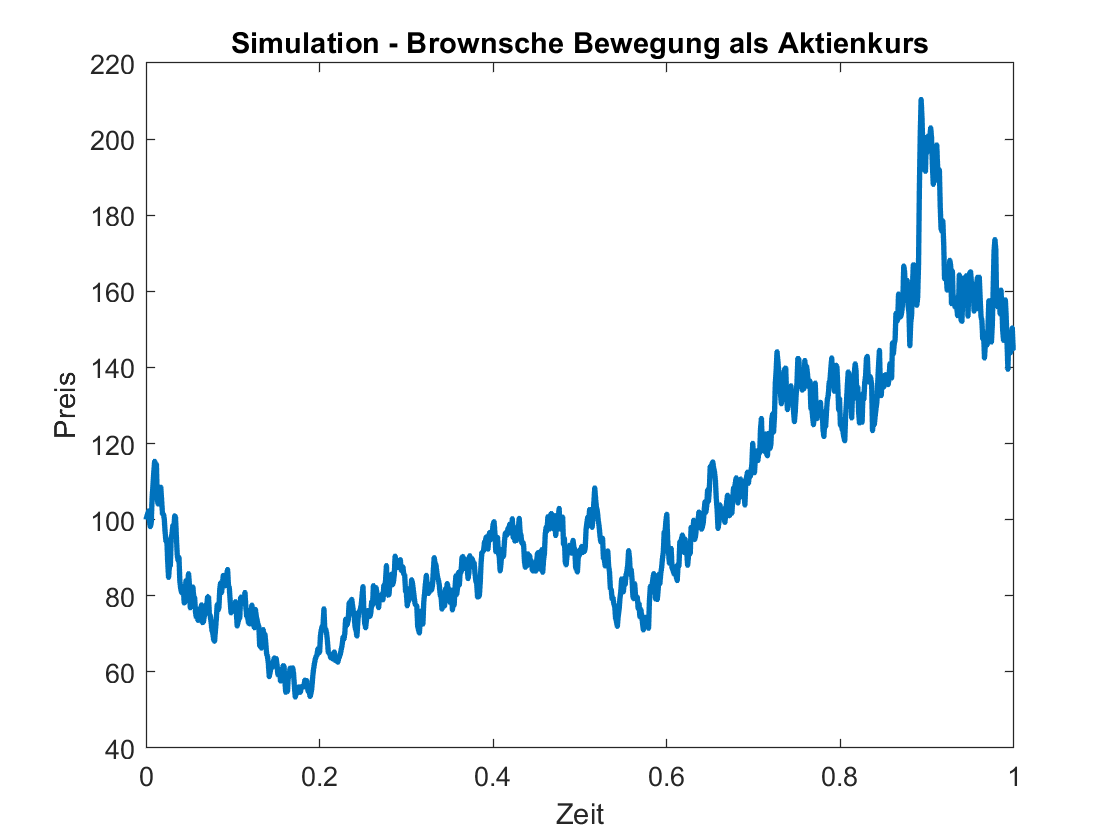
\includegraphics[width=\linewidth]{papers/brown/images/Aktienkurs-als-Brownische-Bewegung_2.png}
		\caption{Stochastisches Rauschen}
	\end{minipage}
	\hspace{0.05\linewidth}
	\begin{minipage}{0.45\textwidth}
		\centering
		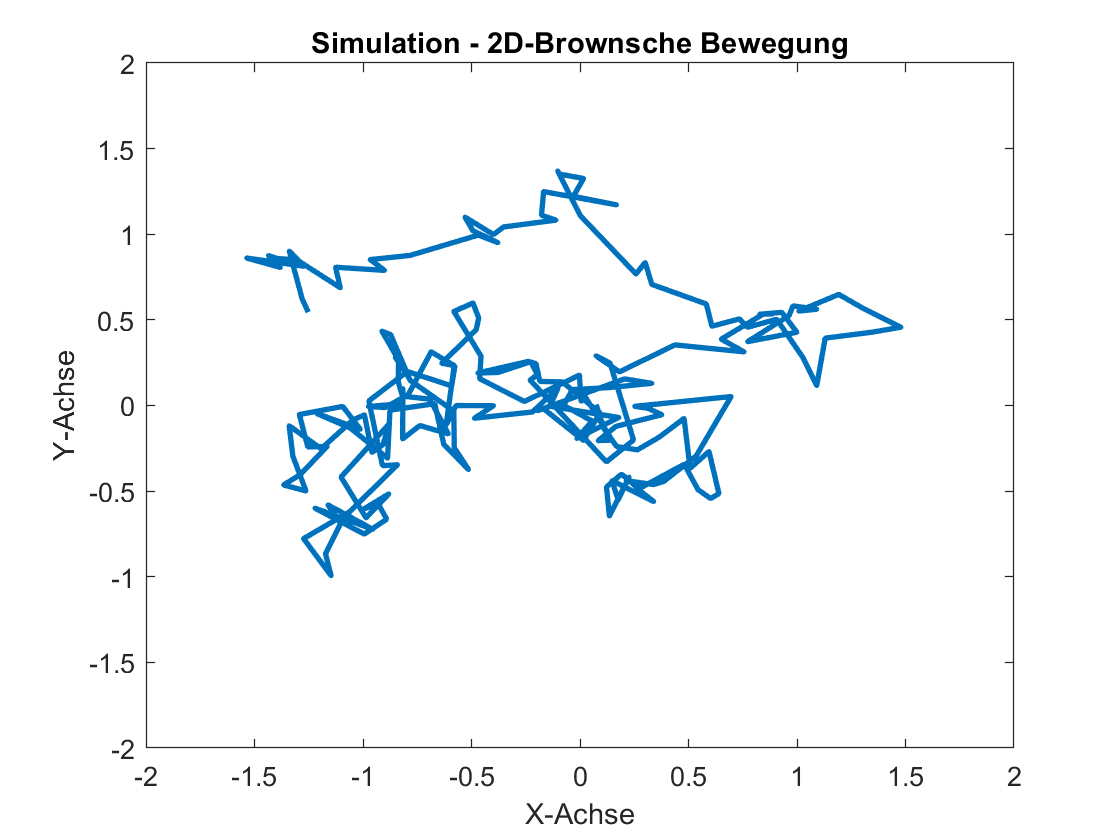
\includegraphics[width=\linewidth]{papers/brown/images/Brownische-Bewegung-Simuliert_2.png}
		\caption{Hochfrequente überlagerte Schwingungen}
	\end{minipage}
\end{figure}


\subsection{Implikationen\label{brown:Rauschen:Implikationen}}
- Faustregel

- Gefahr von Instabilität

- Differnezierbarkeit
\begin{figure}
	\centering
	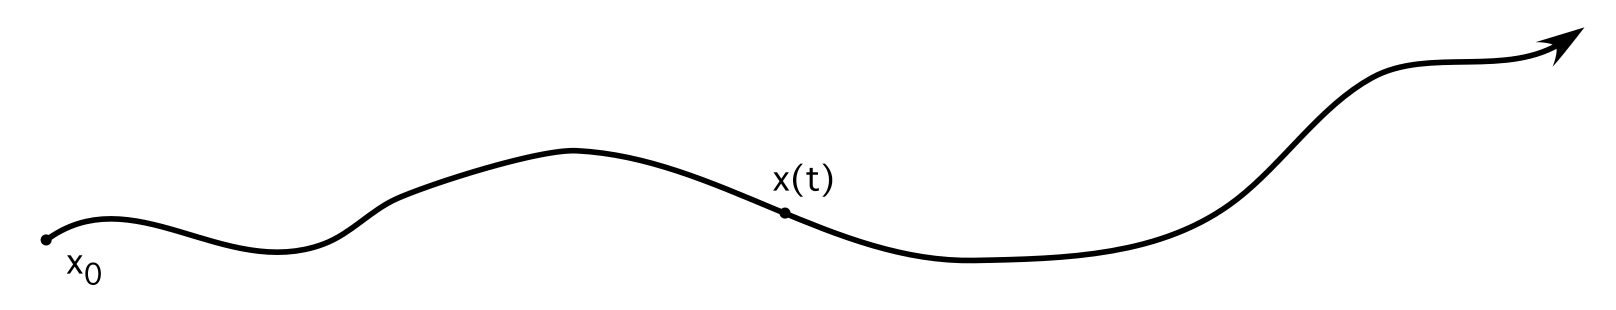
\includegraphics[width=0.3\textwidth]{papers/brown/images/idealSignal.png}
	\caption{Ideales Signal}
	\label{idealSignal}
\end{figure}
\begin{figure}
	\centering
	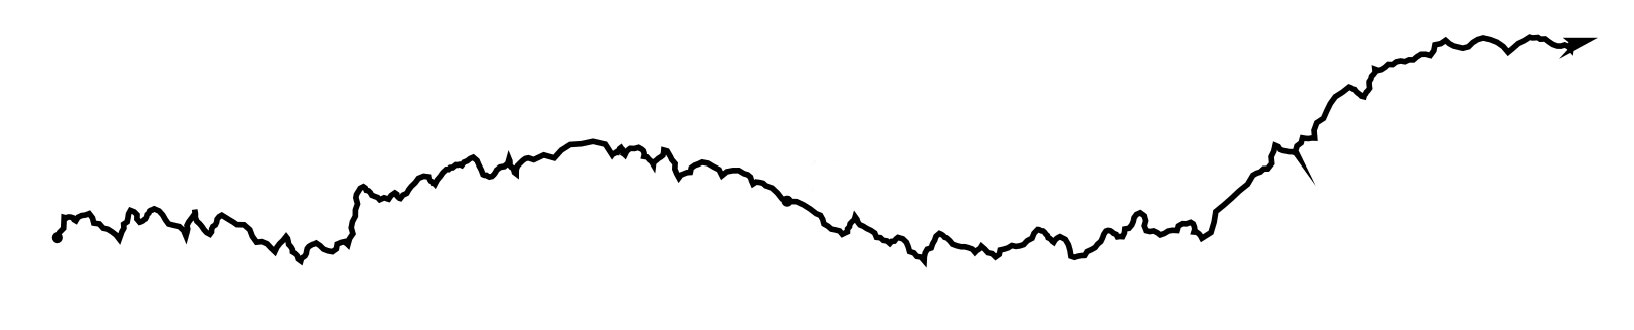
\includegraphics[width=0.3\textwidth]{papers/brown/images/realSignal.png}
	\caption{Reales Signal}
	\label{realSignal}
\end{figure}

Ohne Methoden der stoachstischen Differenzialrechnung kann kaum ein SIgnal anhand von verrauschten Daten oder von zufällig gestörten Systemen erstellt werden. In der Sign